\documentclass{IEEEtran4PSCC}

\usepackage{iftex}
\ifXeTeX\else
  \errmessage{This Chinese translation must be compiled with XeLaTeX}
\fi
\usepackage[UTF8,scheme=plain,heading=false]{ctex}
\usepackage{graphicx}
\usepackage[cmex10]{amsmath}
\usepackage{amssymb}
\usepackage{verbatim}
\usepackage{xurl}
\usepackage{url}
\usepackage{caption}
\usepackage{subcaption}
\usepackage{amsthm}
\usepackage{xcolor}

\renewcommand{\figurename}{图}
\renewcommand{\tablename}{表}
\renewcommand{\proofname}{证明}
\renewcommand{\abstractname}{摘要}
\renewcommand{\IEEEkeywordsname}{关键词}
\renewcommand{\refname}{参考文献}
\renewcommand{\appendixname}{附录}
\providecommand{\appendicesname}{附录}
\newtheorem{thm}{定理}[section]
\newtheorem{prop}[thm]{命题}
\newtheorem{rem}{注}

\makeatletter
\let\old@ps@headings\ps@headings
\let\old@ps@IEEEtitlepagestyle\ps@IEEEtitlepagestyle
\def\psccfooter#1{%
  \def\ps@headings{%
    \old@ps@headings%
    \def\@oddfoot{\strut\hfill#1\hfill\strut}%
    \def\@evenfoot{\strut\hfill#1\hfill\strut}%
  }%
  \def\ps@IEEEtitlepagestyle{%
    \old@ps@IEEEtitlepagestyle%
    \def\@oddfoot{\strut\hfill#1\hfill\strut}%
    \def\@evenfoot{\strut\hfill#1\hfill\strut}%
  }%
  \ps@headings%
}
\makeatother

\psccfooter{%
  \parbox{\textwidth}{\hrulefill\\[-1pt]
  \scriptsize 第24届电力系统计算会议（PSCC 2026）中文翻译版
  \hfill 塞浦路斯利马索尔，2026年6月8--12日}%
}

\begin{document}

\title{构网型变流器的分散式小增益与相位稳定性条件：局限与扩展}

\author{
\IEEEauthorblockN{Diego Cifelli，Adolfo Anta}
\IEEEauthorblockA{奥地利理工学院（AIT Austrian Institute of Technology）\\
奥地利维也纳}}

\maketitle

\begin{center}
\footnotesize
\textbf{非官方中文翻译。}译自 arXiv:2510.20544v2（2026-04-14），未经原作者审校。
翻译属于改编；公式、编号、图及参考文献沿用原版，图内英文未改。
原文：\url{https://arxiv.org/abs/2510.20544v2}；原作采用 CC BY 4.0：
\url{https://creativecommons.org/licenses/by/4.0/}。
\end{center}

\begin{abstract}
随着基于变流器的资源在电力系统中的占比不断提高，稳定性分析亟需无需穷举式全系统仿真的可扩展方法。近期已有研究为此提出分散式小增益与小相位判据，但扇形性假设严重限制了这些判据在构网型变流器中的适用性，因为该假设通常在低频段不成立。本文通过引入环路整形变换，在其他坐标系中重新表述变流器与网络模型，从而重新审视并扩展混合增益--相位条件。所提方法解决了低频固有非扇形性问题并降低了保守性，因而提高了分散式稳定性认证的适用性。本文首先用无限大母线系统说明分析结果，随后将其扩展至 IEEE 14 节点网络，以展示该方法的实用性和可扩展性。这些结果为电网中保守性更低、适用范围更广的分散式稳定性认证提供了路径。
\end{abstract}

\begin{IEEEkeywords}
变流器主导电网；小相位判据；分散式稳定性条件；构网型变流器。
\end{IEEEkeywords}

\thanksto{本研究由 CETPartnership（清洁能源转型伙伴关系）2023 年联合研究提案征集资助，并由欧盟委员会（GA No. 101069750）以及以下机构共同出资：西班牙国家研究署（AEI）、德国 J\"ulich 研究中心项目管理机构（PtJ/MWIKE）、希腊研究与创新总秘书处（GSRI）、爱尔兰可持续能源署（SEAI）、奥地利研究促进署（FFG）和挪威研究理事会（RCN）。}

\section{引言}
现代电力系统中电力电子变流器的渗透率持续提高，电网动态正在发生日益明显的根本变化。基于变流器的资源与既有网络之间的相互作用会产生复杂且尚未得到充分理解的行为。实践中，这类变流器驱动的动态已经引发了意外且不利的现象~\cite{Cigre2024}，凸显出开展系统性稳定性评估的必要性。传统稳定性保障依赖大规模仿真研究；当系统扩展到数百台变流器时，其计算开销往往难以承受，也不再实用。此外，每接入一个新设备都需要重新评估整个系统，进一步加剧了这一挑战。

为克服这些限制，近期研究提出了分散式稳定性判据~\cite{chenExtendedFrequencyDomainPassivity2025a,huangGainPhaseDecentralized2024,häberle2025decentralizedparametricstabilitycertificates}，使单台变流器的影响能够独立于系统中的其他变流器进行评估。这些条件经过设计，使得只要每台变流器分别满足条件，便可保证整个系统稳定，而无需显式分析变流器之间的相互作用。这一范式为变流器主导电网的稳定性认证提供了可扩展、模块化的路径，降低了对穷举式全系统仿真的依赖。同时，这些分散式条件也能为保障系统稳定的变流器控制设计提供有价值的见解。

一种众所周知的分散式稳定性判据要求所有系统元件均具有无源性。该要求已开始出现在即将实施的构网型变流器并网规范中~\cite{fingridGridCode}。网络天然能够满足该条件，但变流器通常不能。在高频段，可通过适当的控制策略强制满足无源性；而在本文所采用的同步 $dq$ 坐标系中，低频非无源性与变流器的恒功率特性内在相关，无法消除。

无源性判据较为保守，后续研究因而提出了更一般、限制更少的框架。文献~\cite{chenExtendedFrequencyDomainPassivity2025a} 及其扩展工作~\cite{chenUnifiedFlexibleFrequencyDomain2025a} 利用无源性指标，使无源设备与非无源设备能够逐频率相互补偿。带权重矩阵的扩展无源性指标提供了更大的灵活性并降低了保守性，但这些方法主要面向单台变流器，尚未扩展到多变流器系统。

文献~\cite{huangGainPhaseDecentralized2024} 基于新的矩阵相位定义，构造了分散式混合增益--相位判据，从而提出另一类更精细的分散式条件。然而，该方法要求变流器导纳满足实际中往往不成立的扇形性条件，限制了其适用范围。文献~\cite{woolcockMixedGainPhase2023} 也针对鲁棒分析提出了类似思路。

为绕开扇形性假设，文献~\cite{baron2025decentralized} 提出基于尺度相对图（scaled relative graph，SRG）的相位计算方法。该方法虽有前景，但构造 SRG 的计算代价较高，而且如何根据黑箱模型计算 SRG 仍是开放问题。

另一项相关研究~\cite{deyPassivityBasedDecentralizedCriteria2023} 在极坐标系中描述系统；在该坐标系下，构网型（GFM）变流器在低频段具有无源性。作者在假设时间尺度分离的基础上提出混合判据：低频段在极坐标系中验证无源性，高频段则采用标准的直角坐标导纳表示。然而，时间尺度分离在实际中未必成立，也可能难以验证。文献~\cite{häberle2025decentralizedparametricstabilitycertificates} 还针对有功--频率（P--f）和无功--电压（Q--V）控制提出了分散式参数化条件，但其适用范围受限于预先规定的控制结构，并忽略了变流器的底层动态。

本文聚焦于文献~\cite{huangGainPhaseDecentralized2024} 提出的分散式小增益/小相位条件。首先，我们指出该方法用于低频增益较高且缺乏扇形性的 GFM 变流器时所面临的局限。随后分析这种非扇形性的来源，说明它源于变流器的恒功率特性，因而无法避免。最后，受文献~\cite{deyPassivityBasedDecentralizedCriteria2023} 启发，我们通过引入环路整形变换扩展文献~\cite{huangGainPhaseDecentralized2024} 的框架，使条件更一般、保守性更低，并解决扇形性问题。

本文其余部分安排如下：第~\ref{sec:gain_phase_crit} 节回顾分散式增益--相位稳定性判据；第~\ref{sec:lim} 节分析其应用于 GFM 变流器时的局限；第~\ref{sec:propo_approch} 节给出本文提出的扩展。第~\ref{sec:ex_1} 节和第~\ref{sec:ex_2} 节分别通过接入无限大母线的变流器和 IEEE 14 节点系统验证所提方法。最后，第~\ref{sec:conc} 节总结全文。

复现本文结果所需的数据和代码见文献~\cite{RepoZenodo}。

\section{混合增益--相位稳定性条件}
\label{sec:gain_phase_crit}

对于矩阵 $A\in\mathbb{C}^{n\times n}$，其 $n$ 个增益定义为各奇异值，其中 $\overline{\sigma}(A)$ 和 $\underline{\sigma}(A)$ 分别表示最大和最小增益。这些量既可以界定 $A$ 的特征值，也可以按照式~\eqref{eq:sv_bound} 界定两个矩阵 $A,B\in\mathbb{C}^{n\times n}$ 乘积的特征值模，而且无需显式计算乘积 $AB$。
\begin{equation}
\underline{\sigma}(A)\underline{\sigma}(B)
\leq |\lambda(AB)|
\leq \overline{\sigma}(A)\overline{\sigma}(B).
\label{eq:sv_bound}
\end{equation}
我们希望为特征值的相位建立类似的界。这个问题更为复杂，直到近期才出现能够导出此类界的矩阵相位定义~\cite{wangPhasesComplexMatrix2020,chenPhaseAnalysisIEEE}。

复矩阵 $A\in\mathbb{C}^{n\times n}$ 的数值域 $W(A)$ 定义为
\begin{equation}
W(A)=\{x^*Ax:\,x\in\mathbb{C}^n,\ \|x\|=1\}.
\label{eq:num_range}
\end{equation}
它是复平面上包含 $A$ 的各特征值的凸子集。若 $W(A)$ 完全位于复平面的某个角扇区内，且 $0\notin W(A)$，则称矩阵 $A$ 为扇形矩阵。对于扇形矩阵 $A$，存在可逆矩阵 $T$，使 $A=T^*DT$，其中 $D$ 是在置换意义下唯一的对角矩阵。$A$ 的相位定义为 $D$ 的对角元的辐角，并按顺序排列，使 $\overline{\phi}(A)$ 和 $\underline{\phi}(A)$ 分别表示最大和最小相位，且 $\overline{\phi}(A)-\underline{\phi}(A)<\pi$。相位区间 $[\underline{\phi}(A),\overline{\phi}(A)]$ 简记为 $\Phi(A)$。该定义还可扩展至拟扇形矩阵（即 $0\in\partial W(A)$）和半扇形矩阵（即 $0\in\partial W(A)$ 且 $\overline{\phi}(A)-\underline{\phi}(A)\leq\pi$）~\cite{chenPhaseTheoryMIMO2022}。

从几何上看，这些相位对应于数值域的角边界。与奇异值完全类似，最大和最小相位可以按照式~\eqref{eq:phase_bound} 界定矩阵乘积特征值的相位：
\begin{equation}
\underline{\phi}(A)+\underline{\phi}(B)
\leq \angle\lambda(AB)
\leq \overline{\phi}(A)+\overline{\phi}(B).
\label{eq:phase_bound}
\end{equation}

\subsection{混合增益--相位稳定性判据}
\begin{figure}
\centering
\begin{subfigure}{0.45\columnwidth}
  \centering
  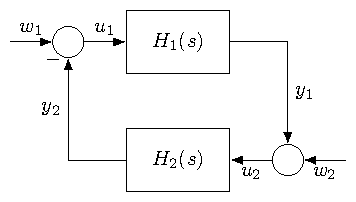
\includegraphics[width=\linewidth]{feedback_diagram.pdf}
  \caption{一般反馈系统。}
  \label{fig:fd_diagram}
\end{subfigure}
\begin{subfigure}{0.45\columnwidth}
  \centering
  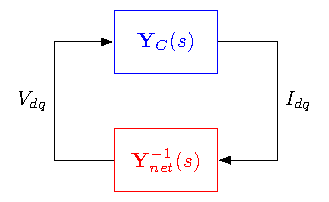
\includegraphics[width=\linewidth]{feedback_diagram_converters_2.pdf}
  \caption{导纳反馈。}
  \label{fig:fd_diagram_conv_net}
\end{subfigure}
\caption{反馈互连示意图。}
\label{fig:twoside}
\end{figure}

上述概念为评估线性时不变系统的稳定性提供了框架。考虑图~\ref{fig:fd_diagram} 所示 $H_1(s)$ 与 $H_2(s)$ 的反馈互连。下述定理给出了所得闭环系统稳定的一个充分条件~\cite{zhao2022smallgainmeetssmall}。

\begin{thm}[混合小增益--相位定理]
设开环系统 $H_1,H_2$ 为实、有理、稳定且真有理的传递函数矩阵。若对每个 $\omega\in[0,\infty]$，下列两项至少有一项成立，则闭环系统稳定：
\begin{enumerate}
\item 最大奇异值之积满足
\begin{equation*}
\overline{\sigma}(H_1(j\omega))\overline{\sigma}(H_2(j\omega))<1;
\end{equation*}
\item $H_1(j\omega)$ 为半扇形矩阵、$H_2(j\omega)$ 为扇形矩阵，且
\begin{equation*}
\overline{\phi}(H_1(j\omega))+\overline{\phi}(H_2(j\omega))<\pi,
\end{equation*}
\begin{equation*}
\underline{\phi}(H_1(j\omega))+\underline{\phi}(H_2(j\omega))>-\pi.
\end{equation*}
\end{enumerate}
\label{thm:mixed_small_gain_phase}
\end{thm}

该定理将传统小增益条件及其相位对应条件统一到同一个稳定性框架中。对每个频率，可以根据哪一种估计较不保守，选择基于增益或相位的界。

\subsection{电力系统稳定性的分散式条件}
\begin{figure}
\centering
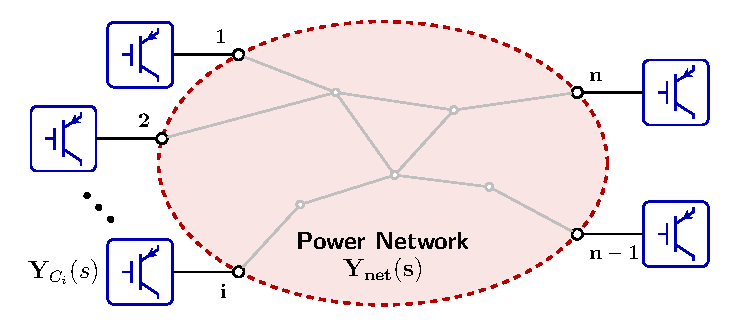
\includegraphics[width=\linewidth]{vsc1.pdf}
\caption{多变流器电力系统示意图。}
\label{fig:multi_converter_diagram}
\end{figure}

在电力系统中，我们关注图~\ref{fig:multi_converter_diagram} 所示 $n$ 台电力电子变流器接入给定网络后的互联系统稳定性。令
\begin{equation}
\mathbf{Y}_C(s)=\operatorname{diag}(Y_{C_1}(s),Y_{C_2}(s),\ldots,Y_{C_n}(s))
\label{eq:block_diagonal}
\end{equation}
表示总体变流器导纳矩阵，其中 $Y_{C_i}(s)$ 为第 $i$ 台变流器的导纳。令 $\mathbf{Y}_{net}(s)$ 表示网络导纳。本文假设 $\mathbf{Y}_{net}(s)$ 已经过 Kron 化简，即消除了所有未接入变流器的内部节点。所有导纳均表示在同一全局 $dq$ 坐标系中。与图~\ref{fig:fd_diagram} 类似，变流器和网络的互连可表示为图~\ref{fig:fd_diagram_conv_net} 所示反馈环路。

可以将定理~\ref{thm:mixed_small_gain_phase} 直接应用于该系统以获得稳定性条件。然而，$\mathbf{Y}_C(s)$ 的块对角结构允许开展分散式稳定性分析，从而得到下述结果~\cite{huangGainPhaseDecentralized2024}。

\begin{thm}[分散式混合小增益--相位定理]
若开环系统稳定，且对每个 $\omega\in[0,\infty]$，下列两项至少有一项成立，则图~\ref{fig:fd_diagram_conv_net} 所示多变流器系统稳定：
\begin{enumerate}
\item 分散式增益条件成立，即
\begin{equation*}
\max_i\overline{\sigma}(Y_{C_i}(j\omega))
<\underline{\sigma}(\mathbf{Y}_{net}(j\omega));
\end{equation*}
\item 分散式相位条件成立，即每个 $Y_{C_i}(j\omega)$ 均为拟扇形矩阵，$\mathbf{Y}_{net}(j\omega)$ 为扇形矩阵，并且
\begin{equation*}
\overline{\phi}(Y_{C_i}(j\omega))
<\pi-\overline{\phi}(\mathbf{Y}_{net}^{-1}(j\omega)),\quad\forall i,
\end{equation*}
\begin{equation*}
\underline{\phi}(Y_{C_i}(j\omega))
>-\pi-\underline{\phi}(\mathbf{Y}_{net}^{-1}(j\omega)),\quad\forall i,
\end{equation*}
\begin{equation*}
\max_i\overline{\phi}(Y_{C_i}(j\omega))
-\min_i\underline{\phi}(Y_{C_i}(j\omega))<\pi.
\end{equation*}
\end{enumerate}
\label{thm:dec_mixed_small_gain_phase}
\end{thm}

这种分散式表述只需检查每台变流器模型的局部条件以及网络模型的条件，便可认证大规模多变流器系统的稳定性，而无需显式计算完整互联系统的动态。

\section{判据用于 GFM 变流器时的局限}
\label{sec:lim}

本节说明定理~\ref{thm:dec_mixed_small_gain_phase} 的稳定性条件为何难以在实际电力系统应用中满足。构网型（GFM）变流器是一个典型例子，因为它通常具有很高的低频增益。为展示这一限制，我们考虑一台采用虚拟同步机（VSM）功率控制的常规 GFM 变流器（详见附录~\ref{apx:GFM_control}），通过短路比较低（SCR 低，即电网阻抗较大）的网络接入无限大母线，见图~\ref{fig:gfm_diag}。所得反馈环路的小增益和小相位曲线如图~\ref{fig:GFM_gain_phase_test} 所示。

该例揭示了三个主要问题：
\begin{itemize}
\item \textbf{违反小增益条件：}变流器增益显著超过电网增益，因此小增益条件始终不能满足。
\item \textbf{违反扇形性：}在 $0.9$ Hz 以下，变流器导纳不具有扇形性，因而不能应用小相位判据。
\item \textbf{保守性：}即使导纳具有扇形性且相位定义良好，在 $50$ Hz 以下，变流器与电网的相位区间也非常接近重叠，并最终在约 $1$ Hz 处发生重叠。这种重叠并不一定意味着系统实际不稳定，而可能只是小相位判据保守性的结果。
\end{itemize}
由此可见，经典小增益与小相位判据在现实的变流器主导场景中存在显著局限。下文进一步分析这种非扇形性的来源。

\begin{figure}[tbh]
\centering
\begin{subfigure}{\columnwidth}
  \centering
  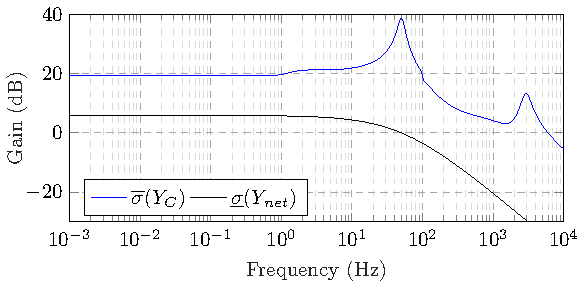
\includegraphics[width=\linewidth]{Gain_adm.pdf}
\end{subfigure}
\begin{subfigure}{\columnwidth}
  \centering
  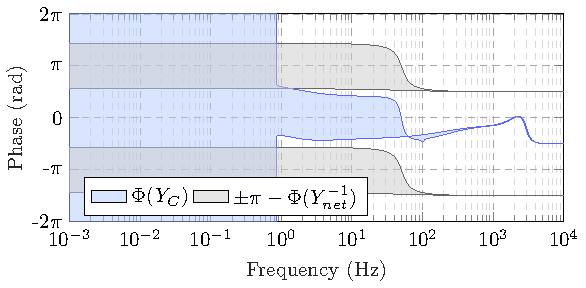
\includegraphics[width=\linewidth]{Phase_adm.pdf}
\end{subfigure}
\caption{GFM 变流器的混合小增益--相位条件。若系统不具有扇形性，则以完整区间 $[-2\pi,2\pi]$ 表示其相位。变流器增益超过网络增益时，小增益条件被违反；变流器相位与平移 $\pm\pi$ 后的网络相位重叠时，小相位条件被违反。}
\label{fig:GFM_gain_phase_test}
\end{figure}

\subsection{GFM 变流器的非扇形性}
如上例及其他研究所示，变流器导纳在低频段经常不具有扇形性~\cite{huangGainPhaseDecentralized2024,woolcockMixedGainPhase2023}。然而，这一现象的来源尚未得到充分研究：它究竟是特定控制架构与参数选择造成的，还是设备本身的固有属性，仍不清楚。

本文采用文献~\cite{guImpedanceBasedWholeSystemModeling2021} 的建模方法。一般变流器的小信号导纳模型如图~\ref{fig:frame_embedding} 所示。模型输入为局部稳态 $DQ$ 坐标系下公共耦合点电压 $V_{DQ}$，输出为同一坐标系下的变流器电流 $I_{DQ}$。变流器控制器工作在局部摆动 $dq$ 坐标系中，在概念上分为两部分：
\begin{itemize}
\item 同步控制器 $K_v(s)$，产生用于将变量从局部稳态坐标系变换到摆动坐标系的角度 $\epsilon$；
\item 其余控制系统 $Y_{dq}(s)$，包括电流控制、电压控制、虚拟阻抗、无功功率控制以及其他与同步无关的控制器。
\end{itemize}
局部稳态坐标系下的闭环导纳可写为
\begin{equation}
Y_{DQ}(s)=(Y_{dq}(s)+I_0^eK_v(s))(I+V_0^eK_v(s))^{-1}.
\label{eq:frame_embedding}
\end{equation}
其中，向量 $V_0^e=[-V_{q,0},V_{d,0}]^T$ 和 $I_0^e=[-I_{q,0},I_{d,0}]^T$ 表示两个坐标系之间旋转关系的线性化项；$V_{d,0},V_{q,0},I_{d,0},I_{q,0}$ 为电压和电流运行点。

\begin{figure}
\centering
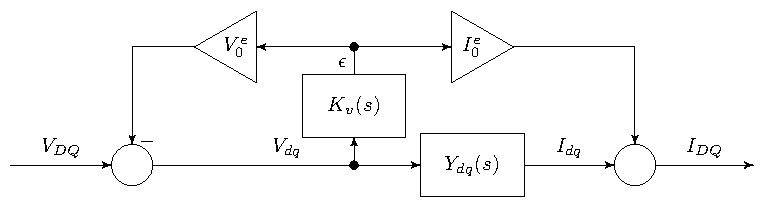
\includegraphics[width=\linewidth]{frame_embedding.pdf}
\caption{嵌入同步坐标系的一般变流器小信号模型。}
\label{fig:frame_embedding}
\end{figure}

对于采用功率同步的典型 GFM 变流器，角度 $\epsilon$ 由式~\eqref{eq:freq_tf} 所示动态系统产生，其中 $\omega$ 为频率，$P$ 为有功功率，$H_P(s)$ 为基于功率的同步环节传递函数：
\begin{equation}
\omega=H_P(s)P,\qquad \epsilon=\frac{1}{s}\omega.
\label{eq:freq_tf}
\end{equation}
对功率表达式线性化得到式~\eqref{eq:power_lin}。其中 $P$ 仅依赖局部稳态坐标系下的电压，因此 $K_v(s)$ 可写成式~\eqref{eq:Kv}：
\begin{equation}
P\approx\underbrace{(V_0Y_{dq}+I_0)}_{:=G_P(s)}V_{dq},\quad
V_0=[V_{d,0}\ V_{q,0}],\quad I_0=[I_{d,0}\ I_{q,0}],
\label{eq:power_lin}
\end{equation}
\begin{equation}
K_v(s)=\frac{H_P(s)}{s}G_P(s).
\label{eq:Kv}
\end{equation}

由于本文关注低频行为，下面考察 $s=j0$ 时的导纳直流增益。关键结果概括如下。

\begin{prop}
假设 $V_{q,0}=0$、$V_{d,0}\neq0$，且 $K_v(s)V_0^e$ 不恒为零。将式~\eqref{eq:Kv} 的 $K_v(s)$ 代入式~\eqref{eq:frame_embedding}，则变流器导纳矩阵在 $s=0$ 时为
\begin{equation}
Y_{DQ}(0)=
\begin{bmatrix}
-\dfrac{I_{d,0}}{V_{d,0}} & -\dfrac{I_{q,0}}{V_{d,0}}\\
\beta & \dfrac{I_{d,0}}{V_{d,0}}
\end{bmatrix},
\label{eq:Y_DQ_0}
\end{equation}
其中 $\beta$ 为某个标量。此外，$Y_{DQ}(0)$ 不具有扇形性。
\label{prop:Y_DQ_0}
\end{prop}

\begin{proof}
式~\eqref{eq:Y_DQ_0} 的推导见附录~\ref{apx:Prop_Y_DQ_0}。由于矩阵迹为零，特征值之和也为零。$2\times2$ 矩阵的数值域是以两个特征值为焦点的椭圆。根据 $\beta$ 和 $I_{q,0}$ 的取值，其长轴为实轴或虚轴。两种情况下原点都属于数值域，因此该矩阵不是扇形矩阵。
\end{proof}

假设 $V_{q,0}=0$ 不失一般性，因为总能选择适当的旋转矩阵使其成立。此外，根据运行点和参数的不同，导纳可能不仅不是扇形矩阵，甚至不是拟扇形矩阵。该结果表明，无论具体控制如何实现，在 $0$ Hz 处都无法实现扇形性，并且在低频段通常也不能满足扇形性。根本原因是 GFM 变流器表现为恒功率负载/电源。即使实施频率下垂控制，使功率随频率变化，从导纳所描述的电压--电流关系看，变流器仍然是恒功率设备。

上述分析还表明，变流器在低频段不是无源的\footnote{此处“无源”采用电力电子文献中常见的宽松逐频率含义，即 $Y(j\omega)$ 的正实性。}。这一结论与文献~\cite{deyAnalysisPassivityCharacteristics2021} 一致，但适用范围更广，因为它不依赖特定的控制实现或参数值。

\begin{rem}
也可以对跟网型（GFL）变流器作类似分析。例如，采用同步旋转坐标系锁相环（SRF-PLL）时，$K_v(s)$ 的形式为 $\frac{H_{PLL}(s)}{s}[0,1]$。对于典型的基于 PI 的有功功率控制，所得导纳与式~\eqref{eq:Y_DQ_0} 具有相同形式。因此，关于低频非扇形性和缺乏无源性的结论同样适用于 GFL 变流器。
\end{rem}

\section{所提方法}
\label{sec:propo_approch}

沿用文献~\cite{deyPassivityBasedDecentralizedCriteria2023,chenExtendedFrequencyDomainPassivity2025a} 的思路，我们指出扇形性并不是系统的固有属性，而取决于输入和输出的具体选择。因此，改用其他变量可能使系统呈现扇形性。

\subsection{功率--极坐标系}
对于 GFM 变流器，一种特别合适的选择是采用功率--极坐标表示：以电压幅值和相位为输入，以有功和无功功率为输出。文献~\cite{deyAnalysisPassivityCharacteristics2021} 表明，这种表示在低频范围内给出 GFM 变流器的无源映射，因此系统具有扇形性。对每台变流器 $i$，相应的线性化变量变换由式~\eqref{eq:change_of_coord_1}--\eqref{eq:change_of_coord_2} 给出，其中变换矩阵 $\mathcal{E}_i$、$\mathcal{F}_i$ 和 $\mathcal{C}_i$ 取决于电压与电流运行点。
\begin{equation}
\begin{bmatrix}
\phi_i\\ |V|_i
\end{bmatrix}
=
\underbrace{
\begin{bmatrix}
-V^i_{q,0} & \dfrac{V^i_{d,0}}{\sqrt{(V^i_{d,0})^2+(V^i_{q,0})^2}}\\
V^i_{q,0} & \dfrac{V^i_{q,0}}{\sqrt{(V^i_{d,0})^2+(V^i_{q,0})^2}}
\end{bmatrix}}_{:=\mathcal{F}_i^{-1}}
\begin{bmatrix}V_{D,i}\\V_{Q,i}\end{bmatrix}.
\label{eq:change_of_coord_1}
\end{equation}

\begin{equation}
\begin{bmatrix}P_i\\Q_i\end{bmatrix}
=\underbrace{\begin{bmatrix}
V^i_{d,0}&V^i_{q,0}\\
V^i_{q,0}&-V^i_{d,0}
\end{bmatrix}}_{:=\mathcal{E}_i}
\begin{bmatrix}I_{D,i}\\I_{Q,i}\end{bmatrix}
+\underbrace{\begin{bmatrix}
I^i_{d,0}&V^i_{q,0}\\
-I^i_{q,0}&I^i_{d,0}
\end{bmatrix}}_{:=\mathcal{C}_i}
\begin{bmatrix}V_{D,i}\\V_{Q,i}\end{bmatrix}.
\label{eq:change_of_coord_2}
\end{equation}

据此，变流器的新输入--输出关系为式~\eqref{eq:pp_trasnf}；网络采用类似变换，得到式~\eqref{eq:pp_trasnf_net}：
\begin{equation}
J_{C,i}(s):=(\mathcal{E}_iY_{C_i}(s)+\mathcal{C}_i)\mathcal{F}_i,
\label{eq:pp_trasnf}
\end{equation}
\begin{equation}
\mathbf{J}_{net}(s):=(\boldsymbol{\mathcal{E}}\mathbf{Y}_{net}(s)-\boldsymbol{\mathcal{C}})\boldsymbol{\mathcal{F}}.
\label{eq:pp_trasnf_net}
\end{equation}
$\boldsymbol{\mathcal{E}}$、$\boldsymbol{\mathcal{C}}$ 和 $\boldsymbol{\mathcal{F}}$ 分别由 $\mathcal{E}_i$、$\mathcal{C}_i$ 和 $\mathcal{F}_i$ 构成块对角矩阵。$\mathcal{C}$ 前的负号源于网络电流方向与变流器中采用的电流方向相反。类似式~\eqref{eq:block_diagonal}，用 $\mathbf{J}_C$ 表示由 $J_{C_i}$ 构成的块对角矩阵。

如图~\ref{fig:loop_shaping} 所示，这一变量变换可以解释为环路变换。假设变换定义良好，则变换前后的输入--输出稳定性等价。系统稳定性由 $\det(\mathbf{Y}_{net}(s)+\mathbf{Y}_C(s))$ 的零点决定；由于
$\det(\mathbf{J}_C(s)+\mathbf{J}_{net}(s))=\det(\boldsymbol{\mathcal{E}}(\mathbf{Y}_{net}(s)+\mathbf{Y}_C(s))\boldsymbol{\mathcal{F}})$，变换前后系统的零点相同。此外，若不存在右半平面极零相消，则输入--输出稳定性蕴含内部稳定性，例如文献~\cite{häberle2025decentralizedparametricstabilitycertificates} 所示。因此，可以无损一般性地将定理~\ref{thm:dec_mixed_small_gain_phase} 直接用于变换后的系统。

\begin{figure}
\centering
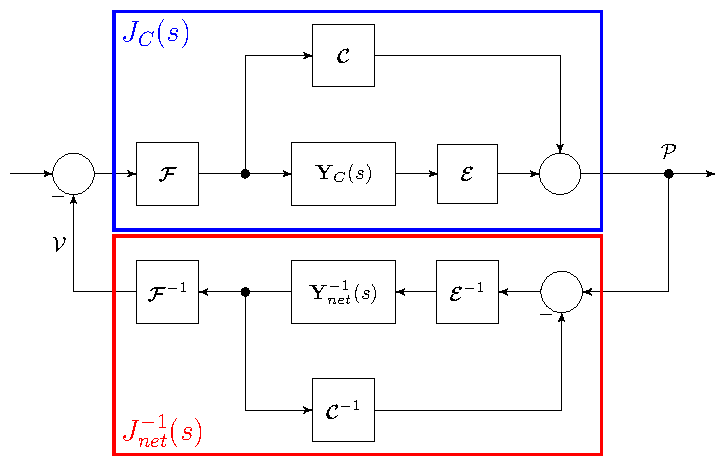
\includegraphics[width=\linewidth]{loop_shaping.pdf}
\caption{将所提变换解释为环路整形变换。}
\label{fig:loop_shaping}
\end{figure}

\begin{rem}
所提变换结合了文献~\cite{woolcockMixedGainPhase2023,chenExtendedFrequencyDomainPassivity2025a,deyPassivityBasedDecentralizedCriteria2023} 中的右乘与整形函数。式~\eqref{eq:pp_trasnf} 同时采用左乘、右乘以及平移项 $\mathcal{C}$。
\end{rem}

对式~\eqref{eq:frame_embedding} 的 GFM 模型应用该变换，直接计算可知 $J_C(s)$ 在零频率处等于式~\eqref{eq:J_C_0}，其中 $\gamma$ 为某个标量。在这种表示中，相位突变不会引起任何稳态功率偏差，电压幅值偏差只会导致无功功率变化。该矩阵为对角矩阵，特征值为 $0$ 和 $\gamma$，数值域是连接这两个特征值的线段。
\begin{equation}
J_C(0)=\begin{bmatrix}0&0\\0&\gamma\end{bmatrix}.
\label{eq:J_C_0}
\end{equation}

在此坐标系中，变流器零频导纳是相位定义良好的拟扇形矩阵。尽管这一性质未必延伸到整个低频段，但它仍是一个积极信号。要应用小相位判据，$\mathbf{J}_C(s)$ 和 $\mathbf{J}_{net}^{-1}(s)$ 必须在整个频率范围内都满足扇形性。该变换可以解决低频非扇形性，却不能保证高频段继续保持扇形性。

为说明这一点，再次分析接入无限大母线的同一台 GFM 变流器。小相位判据结果如图~\ref{fig:pp_frame_cond} 所示。变流器在约 $64$ Hz 以下具有扇形性，并且在这一范围内满足小相位条件。超过该频率后，变流器和网络都不再具有扇形性，判据因而失效。这说明该变换虽然解决了占主导地位的低频限制，却未完全消除小相位方法的适用性限制。

\begin{rem}
尽管 $\mathbf{J}_C(s)$ 继承了 $\mathbf{Y}_C(s)$ 的稳定性，但 $\mathbf{J}_{net}^{-1}(s)$ 未必如此。网络侧变换可解释为反馈运算，因而可能使系统失稳。因此，在应用定理~\ref{thm:dec_mixed_small_gain_phase} 之前，必须验证 $\mathbf{J}_{net}^{-1}(s)$ 的稳定性。
\end{rem}

\begin{figure}
\centering
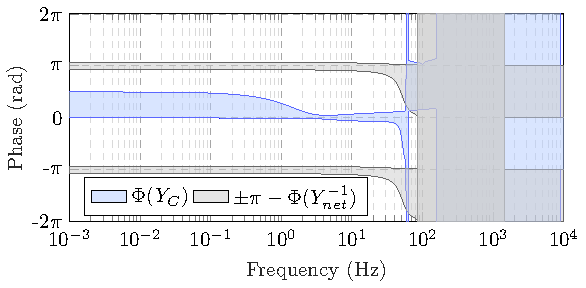
\includegraphics[width=\linewidth]{Phase_polar.pdf}
\caption{功率--极坐标系下 GFM 变流器的小相位条件。}
\label{fig:pp_frame_cond}
\end{figure}

\subsection{统一方法}
如上一节所示，无论采用标准直角坐标导纳系还是功率--极坐标系，相应判据都不能覆盖整个频率范围。在直角坐标系中，高频段（例如 $f>0.7$ Hz）相位定义良好且满足小相位条件；而对于极坐标系下经过环路整形的系统，低频段（例如 $f<64$ Hz）相位定义良好并满足小相位条件。

一种直观做法是组合两种坐标系：高频采用直角坐标系的相位，低频采用极坐标系的相位，只要每个频率上至少有一个坐标系满足小相位判据，就宣布系统稳定。然而，可以构造反例说明，不能简单合并不同坐标系的逐频率结果来推断稳定性。根本原因在于不同变换所界定的量不同：当 $\mathcal{C}$ 不是零矩阵时，$\mathbf{J}_C(j\omega)\mathbf{J}_{net}^{-1}(j\omega)$ 与 $\mathbf{Y}_C(j\omega)\mathbf{Y}_{net}^{-1}(j\omega)$ 的特征值通常并不相同。

为将两种坐标系统一到同一个系统中，令整形矩阵 $\mathcal{E}_i$、$\mathcal{F}_i$ 和 $\mathcal{C}_i$ 成为频率相关矩阵：
\begin{equation}
\begin{aligned}
\tilde{J}_{C_i}(s)&=(\mathcal{E}_i(s)Y_{C_i}(s)+\mathcal{C}_i(s))\mathcal{F}_i(s),\\
\tilde{\mathbf{J}}_{net}(s)&=(\boldsymbol{\mathcal{E}}(s)\mathbf{Y}_{net}(s)-\boldsymbol{\mathcal{C}}(s))\boldsymbol{\mathcal{F}}(s).
\end{aligned}
\label{eq:generic_trasnf}
\end{equation}
这些矩阵的选择必须保证每个 $\tilde{J}_{C_i}(s)$ 以及 $\tilde{\mathbf{J}}_{net}^{-1}(s)$ 均稳定。此外，若 $\boldsymbol{\mathcal{E}}(s)$、$\boldsymbol{\mathcal{C}}(s)$ 和 $\boldsymbol{\mathcal{F}}(s)$ 构成的整形变换适定，则由 $\tilde{\mathbf{J}}_C$ 与 $\tilde{\mathbf{J}}_{net}$ 构成的环路整形系统和由 $\mathbf{Y}_C$ 与 $\mathbf{Y}_{net}$ 构成的原系统具有相同的稳定性。这种表述在选择变换矩阵时十分灵活，但要找到能够同时保证开环稳定性和全频段扇形性的矩阵并不容易。

理想情况下，低频矩阵应与式~\eqref{eq:change_of_coord_1}--\eqref{eq:change_of_coord_2} 中的矩阵一致，以下记为 $\mathcal{E}_{J,i}$、$\mathcal{F}_{J,i}$ 和 $\mathcal{C}_{J,i}$；高频矩阵则应回到直角坐标系，即 $\mathcal{E}=\mathcal{F}=I$、$\mathcal{C}=0$，以下记为 $\mathcal{E}_{Y,i}$、$\mathcal{F}_{Y,i}$ 和 $\mathcal{C}_{Y,i}$。两种状态之间需要连续过渡。以低通/高通滤波为例，$\mathcal{E}_i(s)$ 可采用式~\eqref{eq:freq_dep_tf}，$\mathcal{F}_i(s)$ 和 $\mathcal{C}_i(s)$ 也可作类似处理。滤波器传递函数为 $H_{LPF}(s)=\omega_c/(s+\omega_c)$ 和 $H_{HPF}(s)=1-H_{LPF}(s)$，其中 $\omega_c$ 是截止频率：
\begin{equation}
\mathcal{E}_i(s)=H_{LPF}(s)\mathcal{E}_{J,i}+H_{HPF}(s)\mathcal{E}_{Y,i}.
\label{eq:freq_dep_tf}
\end{equation}
这一变换通常并不合适，因为系统会在滤波器截止频率 $\omega_c$ 附近失去扇形性。

为了在获得紧相位界的同时保证扇形性，本文改用式~\eqref{eq:freq_dep_tf_better} 的变换，并引入附加自由度 $W_i$。该表述只对 $\mathcal{C}(s)$ 与 $\mathcal{F}(s)$ 进行频率相关滤波，而令 $\mathcal{E}(s)$ 保持不变：
\begin{equation}
\begin{aligned}
\mathcal{E}_i(s)&=\mathcal{E}_{J,i},\\
\mathcal{C}_i(s)&=H_{LPF}(s)\mathcal{C}_{J,i},\\
\mathcal{F}_i(s)&=H_{LPF}(s)\mathcal{F}_{J,i}
+H_{HPF}(s)W_i(s)\mathcal{E}_{J,i}^{-1}.
\end{aligned}
\label{eq:freq_dep_tf_better}
\end{equation}
实践观察表明，与式~\eqref{eq:freq_dep_tf} 相比，该变换能在两种坐标系之间产生更平滑的过渡，也更容易保持扇形性。例如令 $W_i(s)=I$，高频时有 $J_{C_i}\approx\mathcal{E}_{J,i}Y_{C_i}\mathcal{E}_{J,i}^{-1}$，从而恢复直角坐标系的性质，因为相似变换不改变数值域。$W_i(s)$ 作为附加权重矩阵还带来更大灵活性，例如可将 $Y_{C_i}(s)$ 中已知的动态转移到 $\mathbf{Y}_{net}(s)$，从而获得更好的扇形行为和更紧的相位界。下一节将用实例说明这一点。当然，其他变换也可能保证扇形性并产生紧相位界；如何寻找最优环路整形变换仍是开放问题。

\section{算例 1：无限大母线}
\label{sec:ex_1}
本节研究如何应用所提方法分析变流器接入前述无限大母线系统时的稳定性。此外，我们还讨论第~\ref{sec:lim} 节所示的保守性问题，以及如何通过适当选择权重矩阵 $W_i(s)$ 缓解这一问题。

\subsection{虚拟导纳补偿}
图~\ref{fig:GFM_gain_phase_test} 表明，即使两个系统都具有扇形性，小相位特征值界在 $50$ Hz 以下仍然非常保守。其原因是 $Y_C$ 和 $Y_{net}^{-1}$ 都具有较大的相位范围。回顾式~\eqref{eq:phase_bound}，小相位界采用最坏情况组合，即最大值与最大值配对、最小值与最小值配对。然而，在乘积 $Y_CY_{net}^{-1}$ 中可能出现有利的相位相互作用，产生部分抵消并减小其特征值相位。图~\ref{fig:phase-bounds_Yv} 清楚展示了这一现象：小相位界 $\Phi(Y_C)+\Phi(Y_{net}^{-1})$ 明显高估了实际特征值相位 $\angle\lambda(Y_CY_{net}^{-1})$。

\begin{figure}
\centering
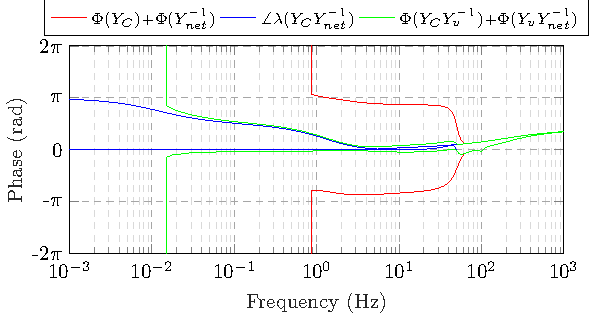
\includegraphics[width=\linewidth]{Phase_Bounds.pdf}
\caption{采用虚拟导纳补偿前后的小相位界。}
\label{fig:phase-bounds_Yv}
\end{figure}

减小数值域的相位张角、限制极端相位组合，可以获得更紧的界。由于变流器实现了虚拟导纳控制 $Y_v(s)$，且其约 $50$ Hz 附近的行为主要由虚拟导纳决定，可以将 $Y_C(s)$ 右乘 $Y_v(s)^{-1}$，使该频段内 $Y_C(s)Y_v(s)^{-1}\approx I$。网络导纳也相应变换为 $Y_{net}(s)Y_v(s)^{-1}$。从另一角度看，这相当于把一项已知动态特性从变流器转移到网络，从而降低保守性。在式~\eqref{eq:freq_dep_tf_better} 中，对应于选择 $W_i(s)=Y_v(s)^{-1}$。

图~\ref{fig:phase-bounds_Yv} 展示了补偿效果。采用所提虚拟导纳滤波后，相位界得到明显改善。乍看之下，这似乎会破坏认证的分散性；但在实践中并不需要精确知道虚拟导纳数值（即约 $50$ Hz 附近的行为），后文将表明近似值已经足够。在分散式场景中，这些数值既可预先选为固定参数，也可由稳定性认证方为不同装置分别指定。无论如何，拟议中的 GFM 并网规范已经给出了有效阻抗的固定范围~\cite{entsoe}。

\begin{rem}
图~\ref{fig:phase-bounds_Yv} 显示，当频率趋于零时，一个特征值的相位趋近 $\pi$。在该频段，小增益条件不能保证 $|\lambda|<1$，稳定性评估因而没有结论。这说明需要引入 $\mathcal{C}$ 所产生的平移，将开环传递函数的特征值移到更合适、可由小相位条件认证稳定性的区域。
\end{rem}

\subsection{完整变换}
图~\ref{fig:phase-dep-frame} 给出了采用频率相关变换~\eqref{eq:generic_trasnf} 后的小相位判据结果，其中矩阵按式~\eqref{eq:freq_dep_tf_better} 定义，滤波器截止频率设为 $0.5$ Hz。与此前结果相比，系统在整个频率范围内都能保持扇形性，并且仅凭小相位条件即可保证闭环稳定。

这意味着该 GFM 变流器的稳定性不依赖以增益衡量的电网强度，在强网和弱网条件下都能保持稳定。从这个意义上说，小相位条件提供了与电网强度无关的稳定性保证。但网络特性变化（如 $R/X$ 比或负荷水平改变）会改变网络相位，可能减小相位裕度并推动变流器趋于失稳。

\begin{figure}
\centering
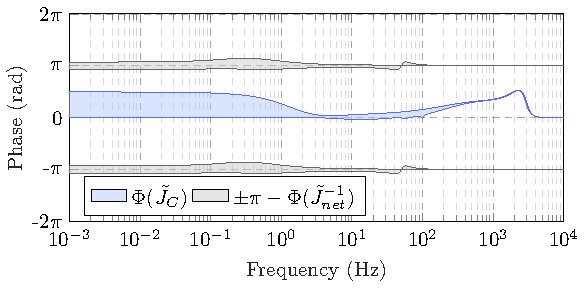
\includegraphics[width=\linewidth]{Phase_mixed.pdf}
\caption{采用式~\eqref{eq:generic_trasnf}、\eqref{eq:freq_dep_tf_better} 的频率相关变换后，GFM 变流器的小相位条件。}
\label{fig:phase-dep-frame}
\end{figure}

\subsection{不稳定情形}
为进一步验证该方法，下面考察定理充分条件的逆否命题：若闭环系统不稳定，则必存在某个频率，使小相位和小增益条件同时被违反。实践中，要使 GFM 变流器失稳并不容易。按照文献~\cite{de2012automatic}，我们在公共耦合点接入纯电阻负载并增大无限大母线阻抗。将控制模式切换为恒无功功率（恒 Q），并把 GFM 的 VSM 阻尼从 $0.5$ 降至 $0.05$ 后，闭环系统失稳，出现 $1.2$ Hz 的持续振荡。图~\ref{fig:GFM_Unstable} 给出了采用所提变换后的混合增益/相位检验结果。

启用无功功率控制会降低低频增益，使小增益条件得到满足。然而，稳定情形（$D=0.5$）满足小相位条件；不稳定情形（$D=0.05$）中，变流器相位显著增大，并与网络相位共同导致相位条件被违反，同时在不稳定振荡频率附近也不满足增益条件。

\begin{figure}
\centering
\begin{subfigure}{\columnwidth}
  \centering
  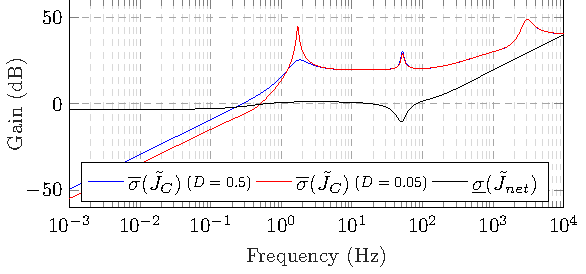
\includegraphics[width=\linewidth]{Gain_inf_un.pdf}
\end{subfigure}
\begin{subfigure}{\columnwidth}
  \centering
  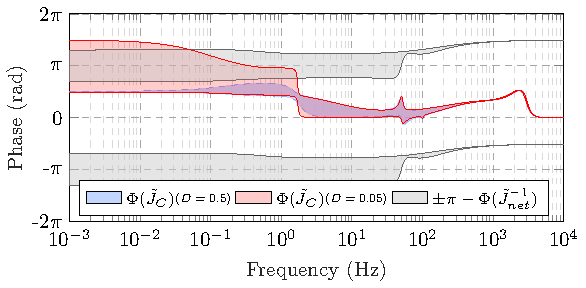
\includegraphics[width=\linewidth]{Phase_inf_un.pdf}
\end{subfigure}
\caption{GFM 接入无限大母线：稳定（$D=0.5$）与不稳定（$D=0.05$）情形对比。}
\label{fig:GFM_Unstable}
\end{figure}

\section{算例 2：IEEE 14 节点系统}
\label{sec:ex_2}
\begin{figure}
\centering
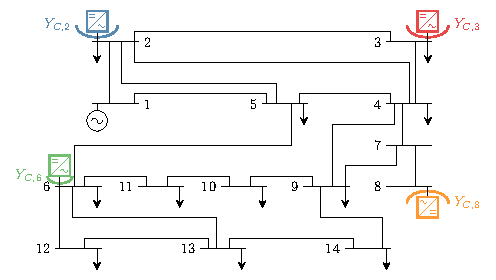
\includegraphics[width=\linewidth]{IEEE14_diagram.pdf}
\caption{IEEE 14 节点系统示意图。}
\label{fig:ieee14_diagram}
\end{figure}

为进一步验证所提方法的可扩展性，本文采用图~\ref{fig:ieee14_diagram} 所示的改进 IEEE 14 节点系统，其参数见文献~\cite{RepoZenodo}。四台 GFM 变流器分别接入节点 2、3、6 和 8。

与无限大母线算例类似，为构造不稳定情形，将变流器 8 的阻尼设为较低值，接入纯电阻负载，并增大线路 7--8 的阻抗。在该配置下，系统发生由变流器 8 驱动的 $0.54$ Hz 不稳定振荡。图~\ref{fig:IEEE14_criteria} 给出了采用所提变换和虚拟导纳补偿后的分散式条件。变流器 2、3 和 6 满足小相位条件，而变流器 8 不满足；具体而言，在 $1.64$ Hz 以下，其相位与网络相位发生重叠。相位重叠本身并不能推出系统不稳定；但在已知系统失稳的情况下，该结果可以识别责任变流器，并可通过适当重调其控制参数恢复稳定。例如，将满足小相位条件的变流器 6 的整定参数用于变流器 8 后，系统即可恢复稳定。

本算例中，各变流器采用不同的虚拟导纳 $R/X$ 比，如表~\ref{tab:virt_adm} 所示；但所有变流器的虚拟导纳补偿均采用固定值 $R_v=0.01$、$X_v=0.1$。这表明即使不知道精确的虚拟导纳，只要采用合理估计，仍可获得适当的相位界，并利用所提方法有效验证稳定性。

\begin{figure}
\centering
\begin{subfigure}{\columnwidth}
  \centering
  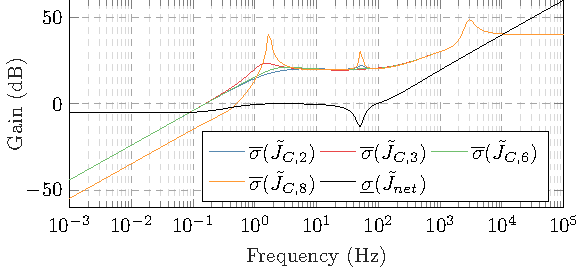
\includegraphics[width=\linewidth]{Gain_14.pdf}
\end{subfigure}
\begin{subfigure}{\columnwidth}
  \centering
  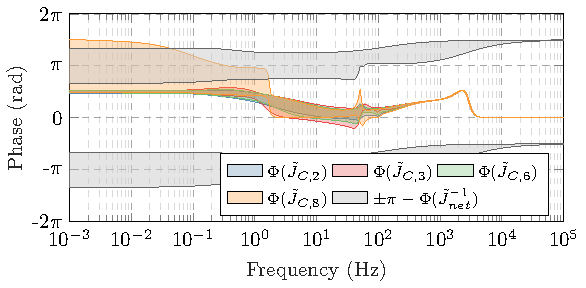
\includegraphics[width=\linewidth]{Phase_14.pdf}
\end{subfigure}
\caption{IEEE 14 节点系统的稳定性分析。}
\label{fig:IEEE14_criteria}
\end{figure}

\begin{table}
\centering
\caption{IEEE 14 节点系统中的虚拟导纳设置。}
\label{tab:virt_adm}
\begin{tabular}{ccc}
GFM 节点 & $R_v$（p.u.） & $X_v$（p.u.）\\
\hline
$2$ & $0.02$ & $0.1$\\
$3$ & $0.05$ & $0.1$\\
$6$ & $0.03$ & $0.1$\\
$8$ & $0.01$ & $0.1$\\
\hline
\end{tabular}
\end{table}

\section{结论}
\label{sec:conc}

本文重新审视了电力系统的分散式小增益--相位条件，并指出其用于 GFM 变流器时的固有局限。为克服这些限制，本文引入一种结合直角坐标导纳系和极坐标导纳系的一般化环路整形变换。该方法不仅解决了变流器的低频非扇形性，还能在整个频率范围内给出更紧的相位行为界。

本文首先在接入无限大母线的 GFM 变流器上演示了该方法，其中虚拟导纳滤波进一步降低了保守性；随后将方法应用于 IEEE 14 节点系统，并成功识别出导致失稳的设备。

尽管结果具有良好前景，仍有若干问题有待解决，特别是系统不仅包含 GFM 变流器，还包含同步机和 GFL 变流器等其他设备时。同步机与本文所研究的 GFM 变流器具有相似动态，因此预计所提方法仍然适用；但励磁器、自动电压调节器和电力系统稳定器等辅助控制环节的影响还需要进一步验证。

对于具有不同动态特性的 GFL 变流器，小增益条件更为关键，所提变换能够带来的收益也较有限。为了给 GFL 装置获得保守性更低的增益条件，一种有益做法是将 GFM 的高增益转移到网络侧，从而提高网络的等效强度。

未来工作将研究变换矩阵的系统化选择方法，并通过把网络拓扑信息嵌入变换来进一步降低保守性。


\bibliographystyle{IEEEtran}
\bibliography{DecCondition_bib}

\appendices
\section{GFM 控制结构}
本文采用图~\ref{fig:gfm_diag} 所示的 GFM 控制结构。控制器在静止 $\alpha\beta$ 坐标系中实现，包括式~\eqref{eq:pr_tf} 给出的比例谐振电流控制器 $PR(s)$，以及式~\eqref{eq:yv_tf} 给出的虚拟导纳电压控制器 $Y_v(s)$，其中 $R_v$ 和 $L_v$ 分别为虚拟电阻和虚拟电感。
\begin{equation}
  PR(s)=K_p+\frac{K_i}{s^2+(2\pi50)^2}
  \label{eq:pr_tf}
\end{equation}
\begin{equation}
  Y_v(s)=\frac{1}{sL_v+R_v},\qquad L_v=\frac{X_v}{2\pi50}
  \label{eq:yv_tf}
\end{equation}
同步控制采用虚拟同步机（VSM），其惯性和阻尼分别为 $H$ 与 $D$。比例积分（PI）控制器通过改变参考电压幅值调节无功功率。除非另有说明，本文禁用无功功率控制器并采用恒定电压幅值参考。参数及更多细节见文献~\cite{RepoZenodo}。

\begin{figure}
  \centering
  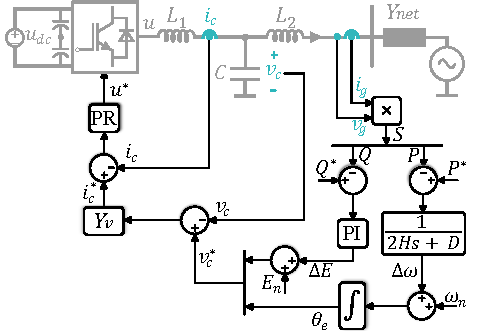
\includegraphics[width=0.9\columnwidth]{drawing.pdf}
  \caption{GFM 控制结构。}
  \label{fig:gfm_diag}
  \vspace{-1em}
\end{figure}
\label{apx:GFM_control}

\section{命题~\ref{prop:Y_DQ_0} 的证明}
\label{apx:Prop_Y_DQ_0}
式~\eqref{eq:frame_embedding} 中的 $Y_{DQ}(s)$ 可改写为式~\eqref{eq:A1}，并进一步化简为式~\eqref{eq:A2}：
\begin{align}
Y_{DQ}(s)&=(Y_{dq}(s)+I_0^eK_v(s))\left(I-\frac{V_0^eK_v(s)}{1+K_v(s)V_0^e}\right)\label{eq:A1}\\
&=Y_{dq}(s)-(Y_{dq}(s)V_0^e-I_0^e)\frac{K_v(s)}{1+K_v(s)V_0^e}.\label{eq:A2}
\end{align}
考虑 $K_v(s)=\frac{H_P(s)}{s}G_P(s)$，并令 $s$ 趋于零，可得
\begin{equation}
Y_{DQ}(0)=Y_{dq}(0)-(Y_{dq}(0)V_0^e-I_0^e)\frac{G_P(0)}{G_P(0)V_0^e}.
\label{eq:A3}
\end{equation}
右乘 $V_0^e$ 后得到 $Y_{DQ}(0)V_0^e=-I_0^e$。也就是说，$Y_{DQ}(0)$ 的第二列乘以 $V_{d,0}$ 等于 $-I_0^e$，与式~\eqref{eq:Y_DQ_0} 一致。通过直接但较繁复的代数运算（为简洁起见略去），还可证明 $Y_{DQ}(0)$ 的 $(1,1)$ 元同样与式~\eqref{eq:Y_DQ_0} 中的相应表达式一致。

\end{document}
